% ============================================================================ VERIFICATION
\section{Verification, Uncertainty and Cost}\label{sec:verification}

A chain of models has no single accuracy, so it is verified by three kinds of check, each of which
establishes something different (Table~\ref{tab:verif}; every check: Table~S17). Each reduced model
is solved together with a reference on the same problem and the same machine
(Fig.~\ref{fig:verif}). The discretization of each FE model is measured on nested refinement
ladders. Model-form choices that no reference can settle are carried as alternatives through the
whole chain (Section~\ref{sec:explore}).

\begin{table}[!t]
\caption{What Each Check Establishes and What It Does Not}
\label{tab:verif}
\centering
\footnotesize
\setlength{\tabcolsep}{2pt}
\begin{tabular}{@{}L{2.45cm}L{2.85cm}L{3.2cm}@{}}
\toprule
Check & Establishes & Does not establish \\
\midrule
Homogenized cards vs explicit unit cells & The mixing rule for the declared pattern & Contact and
intermetallic resistance; full-package accuracy \\
Package networks vs 2-D FE & The DC conduction model as implemented & High-frequency
power-delivery behavior \\
Thermal unit cells vs commercial and open-source FE & The thermal solver on representative cells
& Material data; the cooling boundary \\
Complete package vs open-source FE, identical and refined meshes & The assembled solver input;
the production-mesh error from above & Model form \\
Cold plate vs conjugate CFD & The Nusselt and fin model at the CFD flow & Manifold flow
distribution and header losses \\
Thermoelastic vs closed form and FE; iterative vs direct solver & Element, restraint and
solver tolerance & Solder fatigue \\
Nested mesh ladder of every compared case & Signed bias and $U_{95}$ of each output and
difference & Model accuracy \\
Local mesh family, cycles, dwell, ramp, averaging band; critical-joint search & Discretization
and stabilization; the site that governs & Constitutive validity (carried as a three-law band) \\
Fixed point and energy balance & Convergence and conservation of the coupled solution &
Completeness of the physics \\
Converter model vs circuit simulation~\cite{Abdelzaher2025ECTC,Abdelzaher2026EPEPS} & The loss
model on other members of the family & Accuracy at the synthesized point \\
\bottomrule
\end{tabular}
\end{table}

\subsection{Reference Checks}
The direct-current conduction stages are checked against a commercial thermal FE solver (Ansys
Electronics Desktop, AEDT) through the exact analogy between $\nabla\!\cdot(k\nabla T) = 0$ and $\nabla\!\cdot(\sigma\nabla V) = 0$.
The single-TSV resistance and the TSV-field and attach homogenizations agree with it within
\ErrHomogMax\,\%. The series rule for the through-thickness conductivity of an RDL tier, in
contrast, overstates it by \ErrRdlKz\,\% because it ignores constriction onto the copper grid, so
the reference tensor replaces the rule in every result. The board via field and the solder attach
of Z3 use the same mixing rules as the verified TSV and pillar cards, without a separate
reference. The voltage-fed networks of the Z1 package and of the Z2 ring feed agree with an
open-source FE solution~\cite{MOOSE} to \ErrPkgRdlZone{} and \MthErrRingNet\,\%. The thermal solver
agrees with commercial and open-source FE solutions of representative unit cells to
\ErrThermMax\,\% of the temperature rise.

The complete Z1 package, solved by the production path and by the MOOSE heat-transfer
module~\cite{MOOSE} on the identical mesh of \MthFpElems{} hexahedra, agrees to
\FullPkgErrZone~K at the peak and over the nodal field. The problem used the converged heat map
of the ideal-decoupling case and a uniform film on the plate face. This check verifies the
assembled solver input and solve; Section~\ref{sec:verif-disc} measures the discretization.

The thermoelastic element reproduces the bimaterial closed form~\cite{Timoshenko1925} to
\ErrMechClosed\,\% and a commercial structural solution to \ErrMechAedt\,\%. The direct
structural solver of this CalculiX build~\cite{CalculiX} fails at \MthSolverFailElems{} elements,
so the production meshes use its iterative solver. On the \MthSolverElems-element base mesh the
two solvers agree to \MthSolverDu\,\% in $\du$ but only to \MthSolverWarp\,\% in die warpage.
This solver term lies outside $U_{95}$; added to both cases of every resolved warpage comparison,
it leaves \MthSolverHold{} of them resolved.

A conjugate computational fluid dynamics (CFD) solution of one channel half-pitch
(\MthCfdCells{} cells, constant water properties) checks the plate model at the single-pass flow.
With the three-wall H1 Nusselt number, the correlation is within \MthCfdErr\,\% of the CFD in mean
base temperature rise and within \MthCfdDpErr\,\% in pressure drop.

\begin{figure}[!t]
\centering
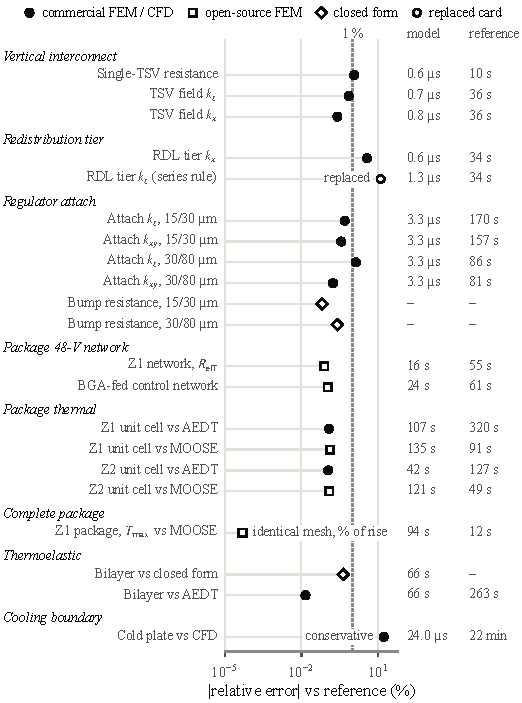
\includegraphics[width=\columnwidth]{fig10_verification.pdf}
\caption{Matched-reference checks: $|$relative error$|$ of each reduced model, and of the
complete Z1 package (CalculiX against MOOSE on the identical mesh), against its reference on the
same problem and machine; right: median runtimes of model and reference. Open marker: the
series-rule RDL conductivity, replaced by the reference tensor in every result; cross: the
iterative against the direct structural solver in die warpage, a term outside $U_{95}$.
Discretization and the local model: Sections~\ref{sec:verif-disc} and~\ref{sec:verif-local}.}
\label{fig:verif}
\end{figure}

\subsection{Discretization and the Resolution Rule}\label{sec:verif-disc}
The package mesh is a graded 1.1-mm grid refined by nested splitting, in which every coarse node
survives; level r$IJ$ splits every in-plane interval into $I$ and every layer into $J$ parts.
Splitting every in-plane interval in two changed the Z1 peak temperature by \MthMeshStepT\,\%, so
the production mesh is r21 (Table~S16). Every compared case, Z1--Z3 under both coolings in the
production state, carries its own ladder of three in-plane levels, r11, r21 and r31. The
ideal-decoupling references of Z1 and Z2 add a through-thickness rung, r12.

MOOSE solutions of the complete Z1 package on uniformly refined copies of up to
\MthFpMaxElems~M hexahedra measure the production-mesh error from above. The die is converged to
\MthFpDie~K. The converter stack, substrate, BGA and board are \MthFpLayerLo--\MthFpLayerHi~K
too cold, converging at an observed order of only \MthFpOrder, and the peak is \MthFpErr~K too
low. The in-plane resolution of the cells causes this error: through-thickness refinement alone
moves the peak by \MthFpTt~K of the \MthFpX~K of a full doubling. For the same case, the bias
plus $U_{95}$ of the production ladder reaches \MthFpBandHi~K and contains this error.

A difference $D = y_b - y_a$ between two cases is \emph{resolved} when $|D+\beta_D| > U_{95}(D)$.
The signed bias $\beta_D$ and the discretization term come from a grid-convergence-index (GCI)
estimate on $D$'s own rung sequence~\cite{Roache1998,Celik2008}. Errors that the two cases share
on one mesh family thus cancel only where they move together. A monotone ladder whose observed
order lies within 0.2 of the formal order 2 is asymptotic and uses the safety factor
$F_s = 1.25$. Other monotone ladders use $F_s = 3$ with the order limited to [0.5,~2]. An
oscillatory ladder carries $F_s$ = 3 times half its range and no signed bias. The bias is
$\beta = e_{32}r^p/(r^p-1)$, with $e_{32}$ the r21-to-r31 change, $p$ the order and $r = 1.5$.

$U_{95}(D)$ adds three terms in quadrature to the discretization term: the through-thickness
split where an r12 rung exists, the fixed-point stop of each case (0.1\,\% of the loss,
0.25~K) and the matched-reference agreement of the solver (0.13\,\% of a temperature
difference, 0.43\,\% of a displacement difference). The coverage is about 95\,\%. Model-form
uncertainty is not part of $U_{95}$. Section~\ref{sec:explore} evaluates both integrations under
each declared alternative, and a resolved ranking that an alternative reverses is conditional on
it.

Of the \MthNcomp{} compared differences in loss, peak temperature, warpage and $\du$
(Table~\ref{tab:uncertainty}; per-case values: Table~S18), \MthNasymWord{} have asymptotic ladders,
\MthNnotasym{} monotone but not asymptotic ones and \MthNoscWord{} oscillatory ones. The rule resolves
\MthNresolved{} of them; only the loss of Z3 against Z1 under cooling~B is not resolved. The
production mesh underestimates every loss, by \MthBiasPLo--\MthBiasPHi~W, and every peak
temperature, by \MthBiasTLo--\MthBiasTHi~K. Testing each difference on its own ladder matters:
under cooling~A, the \GapAZtwo-W loss gap between Z1 and Z2 has $U_{95}(D) =
\WrResAZoneZtwoPlossUni$~W, whereas the two cases' own $U_{95}$ sum to \MthGapAPlossSum~W.

The through-thickness term is measured on the ideal-decoupling references. It moves loss and
peak temperature by at most \MthTtTZone\,\%, but the die warpage of Z1 by \MthTtWarpZone\,\% and
its $\du$ by \MthTtDuZone\,\%. The production ladders lack this rung. Adding the relative term of
the references to every compared case, together with the solver term to every warpage, leaves
\MthTtHold{} resolved differences resolved; the die warpage of Z3 against Z1 under cooling~B is the
exception.

The coupled solution conserves energy. Heat deposited in the mesh equals the ledger total to
round-off (a relative $\MthDepositResid$), and heat leaving through the plate and board films
equals the deposited heat to a relative $\MthEnergyResid$ in every compared case.

\subsection{Local Response and Critical Joint}\label{sec:verif-local}
The local model is verified at the critical joints of the production state (Tables~S12--S14).
Refining its mesh from L0 to L3 changes the six responses by at most \MvMeshUmax\,\%, and eight
cycles leave the four-cycle responses unchanged at the printed precision, so their numerical
$U_{95}$ is at most \MvMeshUmax\,\%. A 60-s or 900-s dwell changes the responses by
\MvDwellSixtyLo{} to \MvDwellNineHundredHi\,\%, and a 30-s ramp by at most \MvRampThirtyHi\,\%;
neither changes a ranking. The averaging core excludes a corner band of
\MthBandProdUm~\textmu m; bands of \MthBandUm~\textmu m, at L0 and L2, change the responses by
\MthBandLo{} to \MthBandHi\,\% and no ordering. The two band laws give
\MvRatioXiaoLo--\MvRatioXiaoHi{} and \MvRatioMeasLo--\MvRatioMeasHi{} times the response of the
production law, and under each law the critical joint is the same site.

The critical-joint search terminated in every case with no unsolved site bounded above the
largest response (Table~S13). Of the \MvCritLattice{} lattice sites of the six cases, it solved
\MvCritSchubSolved{} under the production law and \MvCritSolvedAll{} under the three laws. The
screening features are needed because the response is not monotone in the in-plane displacement
and the joint temperature. In \num[group-separator={,}]{\MvCritViol} of \MvCritPairs{} pairs of
sites ordered by $(\Delta u, T_{\mathrm{sj}})$, the dominated site responds more, by up to
\MvCritViolMax\,\%. In the screening features only \MvCritViolF{} of \MvCritPairsF{} ordered
pairs reverse by more than 1\,\%, by at most \MvCritRevF\,\%, which sets the margin at
\MvCritMarginMin--\MvCritMargin\,\%.

The joint of largest $\Delta u$, or its mirror image within the 1-\% noise of the local model, is
the critical joint in every case except those of Z2. Under cooling~A, the critical joint of Z2 is
an inner site of the ring that responds \MvCritRatioMax\,\% more than the joint of largest
$\Delta u$. Under cooling~B, it is the mirror corner, which responds \MvCritRatioBZtwo{} times as
much because the streamwise coolant breaks the symmetry.

% GENERATED by scripts/tcpmt_uncertainty.py -- do not edit
\begin{table}[!t]
\caption{Numerical uncertainty $U$ of each compared output (S0, production mesh) and the comparisons it resolves: a gap is resolved when it exceeds $2(U_a+U_b)$.}
\label{tab:uncertainty}
\centering
\footnotesize
\setlength{\tabcolsep}{2.5pt}
\begin{tabular}{@{}lrrrrrr@{}}
\toprule
 & \multicolumn{3}{c}{Cooling A: $\pm U$} & \multicolumn{3}{c}{Cooling B: $\pm U$}\\
\cmidrule(lr){2-4}\cmidrule(l){5-7}
Output & Z1 & Z2 & Z3 & Z1 & Z2 & Z3 \\
\midrule
Loss (W) & 0.67 & 0.62 & 0.78 & 0.67 & 0.48 & 0.49 \\
Peak temp.\ (K) & 1.36 & 0.97 & 1.22 & 1.30 & 0.55 & 0.44 \\
Die warpage (\textmu m) & 0.62 & 0.69 & 3.08 & 0.14 & 0.18 & 0.37 \\
$\du$ (\textmu m) & 0.04 & 0.06 & 0.18 & 0.01 & 0.04 & 0.06 \\
$\deps$ ($10^{-3}$/cycle) & 0.19 & 0.25 & 1.63 & 0.04 & 0.03 & 0.30 \\
\midrule
\multicolumn{7}{@{}l}{\emph{Comparisons (lower first; R: resolved, --: within $2U$)}}\\
\multicolumn{7}{@{}p{0.95\columnwidth}@{}}{A, Z1/Z2: Loss Z1 R; Peak temp.\ Z1 R; Die warpage Z1 R; $\du$ Z1 R; $\deps$ Z1 R}\\
\multicolumn{7}{@{}p{0.95\columnwidth}@{}}{A, Z1/Z3: Loss Z1 R; Peak temp.\ Z1 R; Die warpage Z1 R; $\du$ Z1 R; $\deps$ Z1 R}\\
\multicolumn{7}{@{}p{0.95\columnwidth}@{}}{B, Z2/Z1: Loss Z2 R; Peak temp.\ Z2 R; Die warpage Z1 R; $\du$ Z1 R; $\deps$ Z1 R}\\
\multicolumn{7}{@{}p{0.95\columnwidth}@{}}{B, Z3/Z1: Loss Z3 R; Peak temp.\ Z3 R; Die warpage Z1 R; $\du$ Z1 R; $\deps$ Z1 --}\\
\multicolumn{7}{@{}p{0.95\columnwidth}@{}}{B, Z2/Z3: Loss Z2 R; Peak temp.\ Z2 --; Die warpage Z3 R; $\du$ Z3 R; $\deps$ Z3 R}\\
\bottomrule
\end{tabular}
\end{table}


\subsection{Cost}
The analytical stages cost microseconds to minutes. A homogenized card takes microseconds
(Fig.~\ref{fig:verif}), the converter cards of a design \MthCardsSec~s, the tier-order search
\MthTierOrderMin~min and the \FrDseNcounts-count electrical screen \MthDseMin~min. One coupled
evaluation on the production mesh, without the local model, takes \MthTotHLo--\MthTotHHi~h on a two-socket
workstation (Intel Xeon Gold 6342; CalculiX~2.23). The electrothermal fixed point takes
\MthEtMinLo--\MthEtMinHi~min for \MthEtItersLo--\MthEtItersHi{} thermal solves on two threads.
The structural solve with the all-site search takes \MthMechMinLo--\MthMechMinHi~min on one
thread, and geometry and meshing take under 2~min. The critical-joint search adds
\MvCritSolvedAll{} independent solves of the local model over the six cases and three laws; they
parallelize over the sites. The per-stage breakdown, mesh sizes, degrees of freedom and peak
memory are in Table~S16. On the identical package mesh the open-source solver is faster (\FullPkgMooseZone~s
against \FullPkgCcxZone~s on eight cores), because the production path factors the system with a
single-threaded direct solver.
